\documentclass[9pt, titlepage]{extarticle}
\usepackage{wrapfig}
\usepackage{lipsum}
\usepackage[utf8]{inputenc} % allows UTF-8, support special characters
\usepackage[UKenglish]{babel} % use UK English hyphenation rules
\usepackage{csquotes} % recommended by babel, better quotes
\usepackage[a4paper, margin=2.15cm]{geometry} % smaller margins, see below

\usepackage[style=numeric, sorting=none]{biblatex}

\usepackage{graphicx} % allows images
\usepackage{hyperref} % automatically links references within the document

\addbibresource{ref.bib} % links bibiography file

\renewcommand*{\bibfont}{\small}
\setlength\bibitemsep{1mm}

\usepackage{tabularx}
\usepackage{enumitem}

\setlength{\parindent}{0pt}

\title{Planning and Design Document}
\author{
\LARGE{
\textbf{Group 32} \\\\
Module Organiser: Dr. James Archbold \\
Tutor: Mahshid Mehr Nezhad \\\\
Alexander Price \\
Thomas Cowley \\
George Denny \\
Yang Tang \\
Moustafa Eladawy
}}
\date{January 2021}

\begin{document}
    %\maketitle
    %\tableofcontents
    %%\newpage

\Large{
\emph{Design and Planning Document, Group 32}
\hfill
February 2021}
\normalsize{}

\section{Introduction}

The stakeholders require an event interaction system that makes use of live feedback to derive event-related metrics.
This document details the proposed system's design, and how this design meets the needs and requirements derived from the specification in `Requirements Analysis'. 
This design document is to be read by the stakeholders, the development team, and the assessor (Dr. James Archbold).
% \begin{tabular}{| l l }
%     \textbf{Version} & \textbf{Changes}\\
%     {\hspace*{1mm}v1.0} & First draft generated
% \end{tabular}
% \vspace*{-2mm}
\section{Glossary}

\begin{tabularx}{\linewidth}{ l X }
    % \emph{Event:}       & An instance that connects participants to a host, representative of a real world event.
    %                     Events are started by hosts and persists until closed by the hosts. \\
    %  \emph{Feedback:}    & Real time evaluative or corrective information about a live real world event; 
    %                     generated by participants and sent to hosts through the solution.\\
    % \emph{Participant:} & A user type. 
    %                     participants attend events and can submit feedback to the event host.\\
    % \emph{Hosts:}       & A type of user, they create, edit, and run events. 
    %                     During events they receive feedback from participants. 
    %                     They can view feedback from all events they have run.\\
    %\emph{Template:}    & A predefined format storing user feedback; 
    %                    this is submitted by the user.\\
    % \emph{Mute:}        & A relationship between a host and a participant, where the participants instances of feedback are not viewable by the host. 
    %                     Their feedback is still used to determine mood.\\
    % \emph{Anonymous:}   & A participant state preventing hosts from viewing their feedback.\\
    % {Template:}         & A framework for feedback, structured with form components.\\
    % % & A feedback framework allowing for structured submission.\\
    % {Generic event:}    & Common real-world events for which the solution is likely to be used.\\
    %                     % Some features will be designed specifically for one or more generic event type.\\
    % {Sentiment:}        & An estimate of the overall opinion/s of a particular instance of feedback.\\
    % {Mood:}             & An estimate of the overall opinion/s of a group of feedback instances.\\
    {NLP:}     & Natural Language Processing\\
    {REST:}     & Representational state transfer (protocol)\\
    {POST/ GET:} & Data request methods over HTTP, methods of REST-APIs\\
    {API:}     & Application Programming Interface\\
    {UI:}      & User Interface\\
    {SCn:}      & Sprint Cycle number n\\
    {R:X.X.X:}      & A reference key for a requirement from the Requirements Analysis document (example R:17.2.D).\\
\end{tabularx}

\section{Solution Overview and Justification}

The client platforms on which the system will be accessible are web, and mobile (Android and iOS). This fulfills [R:1], see Front-end for implementation. \\

\textbf{Front-end}\\
The web-app will use the front-end framework React-JS \autocite{web:react}. 
React-JS is a labour economical framework to create interactive UIs for web applications. React apps use JavaScript to define various `components` which are used to dynamically build the page. This splits up the UI into re-usable components that will improve the maintainability of the code. Accessing server-related data is more efficient in React than in alternative technologies such as the HTML5 stack. React will store data for each component's current state as variables in memory, so data retrieval and updates can be performed more quickly and more succinctly than traditional technologies. The solution will be developed with TypeScript \texttt{v4.1} \autocite{web:ts} over plain JavaScript \autocite{web:js}. TypeScript is a strongly-typed super-set of JavaScript, meaning that type correctness will be checked at compile-time - this avoids type errors during run-time, making the system more robust. TypeScript files compile to JavaScript files to be used in deployment. \\

The project's mobile platforms - Android and iOS - will use React Native \autocite{web:react-native}, a framework for building native apps in React \autocite{web:react}. This allows for code re-use between the web front-end and the mobile front-end, accelerating the rate of development and improving cross-platform design consistency. \\

\textbf{Back-end and Data Storage}\\
All front-end clients interact with a shared back-end implemented in Spark \autocite{web:spark}, a Java framework.\\

Java \texttt{v11.0.9} \autocite{java} is the chosen back-end language of the system. 
Java's object oriented structure composes the system back-end in a logical manner.
Java is also strongly-typed, decreasing run-time errors and increasing the speed of development. Java supports concurrency, which if implemented, provides a more responsive back-end system. Spark was chosen as the Java back-end framework due to both its superior documentation (allowing for accelerated development), and its open license use policies. Further to this, Spark has fast data access speeds since it uses an in-memory (RAM) computing system. \\

The system will organise and store system data, such as events, feedback, and users, in a postgreSQL (pSQL) \autocite{web:psql} database. A structured query language was chosen over alternatives such as NoSQL as its relational model better suits the logical structure of data within the system. SQL is also a non-procedural language, which allows for the simultaneous accessing of multiple records. Furthermore, SQL can easily be embedded in Java using JDBC \autocite{jdbc}. pSQL was chosen due to its open-source and community-driven nature, its close adherence with SQL standards, and its ease of extensibility. \\

\textbf{Sentiment Analysis} 

VADER \autocite{vader2} (Java version) \autocite{web:vader}, the open source empirically derived lexicon and rule-based sentiment analysis tool, will be used instead of creating a comprehensive sentiment lexicon from scratch. 
The project is constrained by time and labour limits, and no developer has any experience with NLP - therefore using an existing framework would be less labour intensive and produce better results.
Other open source NLP frameworks such as spaCy, NLTK, PyTorch, and OpenNLP were also considered. These were found to be less powerful then VADER (during prototyping), which was able to correctly analyse complex qualitative statements and informal language, whereas alternatives struggled in these areas.\\

\section{User Interaction Modelling}

\subsection{Page Structure}

For an understanding of the solution's authentication system, see \autoref{auth}.

\begin{itemize}[noitemsep]
    \item \texttt{/index}: The landing page for the application; users can select either to join an event, or to sign in as a host.
    \item \texttt{/event/join/<eventCode>}: The participant-facing event page in which participants can submit feedback and view event-related information. Participants leave by choice or following event closure by the host. See \autoref{fig:event_ui}. This fulfills [R:3.1], [R:3.3], and [R:3.4].
    \item \texttt{/host/login}: Users can either login as a host, or select to generate a new host account with their email address. This fulfills [R:2].
    \item \texttt{/host/get-code}: Hosts enter their email to generate their host code  (generated upon email verification). This fulfills [R:2].
    \item \texttt{/host/home}: The host's `dashboard'. Hosts can create events, view/edit their created templates, or log out.
    \item \texttt{/host/create-event}: The event-creation page, hosts specify event properties such as the title, and template.
    \item \texttt{/event/host/<eventCode>}: The host-facing event page. Hosts can view participant feedback (including sentiment). Hosts can also view event related metrics such as real-time mood, mean mood, and mean mood over time. Hosts are able to view the event codes for distribution. Hosts can terminate said event. This fulfills [R:13.1-3].
    \item \texttt{/host/templates}: This page lists all templates - both the host's own created templates (to be edited, duplicated, or viewed) and built-in templates (to be viewed or duplicated). Hosts can also create new templates. This fulfills [R:11.2].
    \item \texttt{/host/templates/new}: In this page the host specifies the name of the new template to be created.
    \item \texttt{/host/templates/edit/<templateCode>}: The interface for the solution's template creation system. The host can edit a template by selecting (system predefined) form components. See \autoref{fig:template_ui}. This fulfills [R:11.1] and [R:11.3].
\end{itemize}

\begin{figure}[h!]
\centering
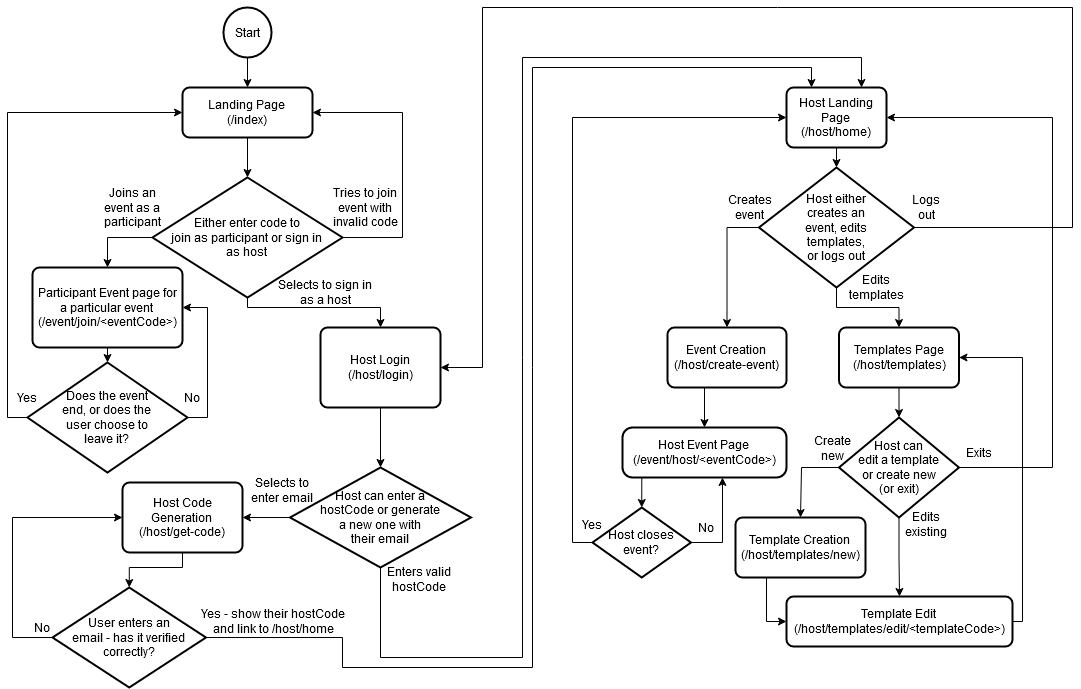
\includegraphics[width=0.95\textwidth]{assets/flow-new.png}
\caption{Front-end user interaction flow-chart, created with Diagrams.net \autocite{web:drawio}.}
\label{fig:flow_diagram}
\end{figure}

\autoref{fig:flow_diagram} represents the paths of interactions exposed to the user by the system front-end. 
Rectangles represent pages, diamonds represent decisions the user can make, and arrows represent paths between resources (pages). 
The user-interaction diagram is divided into two main paths based on the user being a participant, or a host. \newline

Consider the case of a host creating and hosting an event. The host arrives on the landing page, and chooses to sign in as a host. On \texttt{/host/login}, they enter their host code (generalised as \texttt{<}hostCode\texttt{>}), which brings them to \texttt{/host/home} where they choose between hosting an event and editing a template. In the case where this host first creates a template, the host goes to \texttt{/host/templates}, then \texttt{/host/templates/new}, then \texttt{/host/templates/edit/<templateCode>}, where they create said template. Following template creation, the host navigates back to \texttt{/host/home}, then to \texttt{/host/create-event} for event creation. The host-facing event page is launched on \texttt{/event/host/<eventCode>}.

\subsection{Event Sequence Diagram}

\begin{wrapfigure}[17]{l}{0.62\textwidth}
\centering
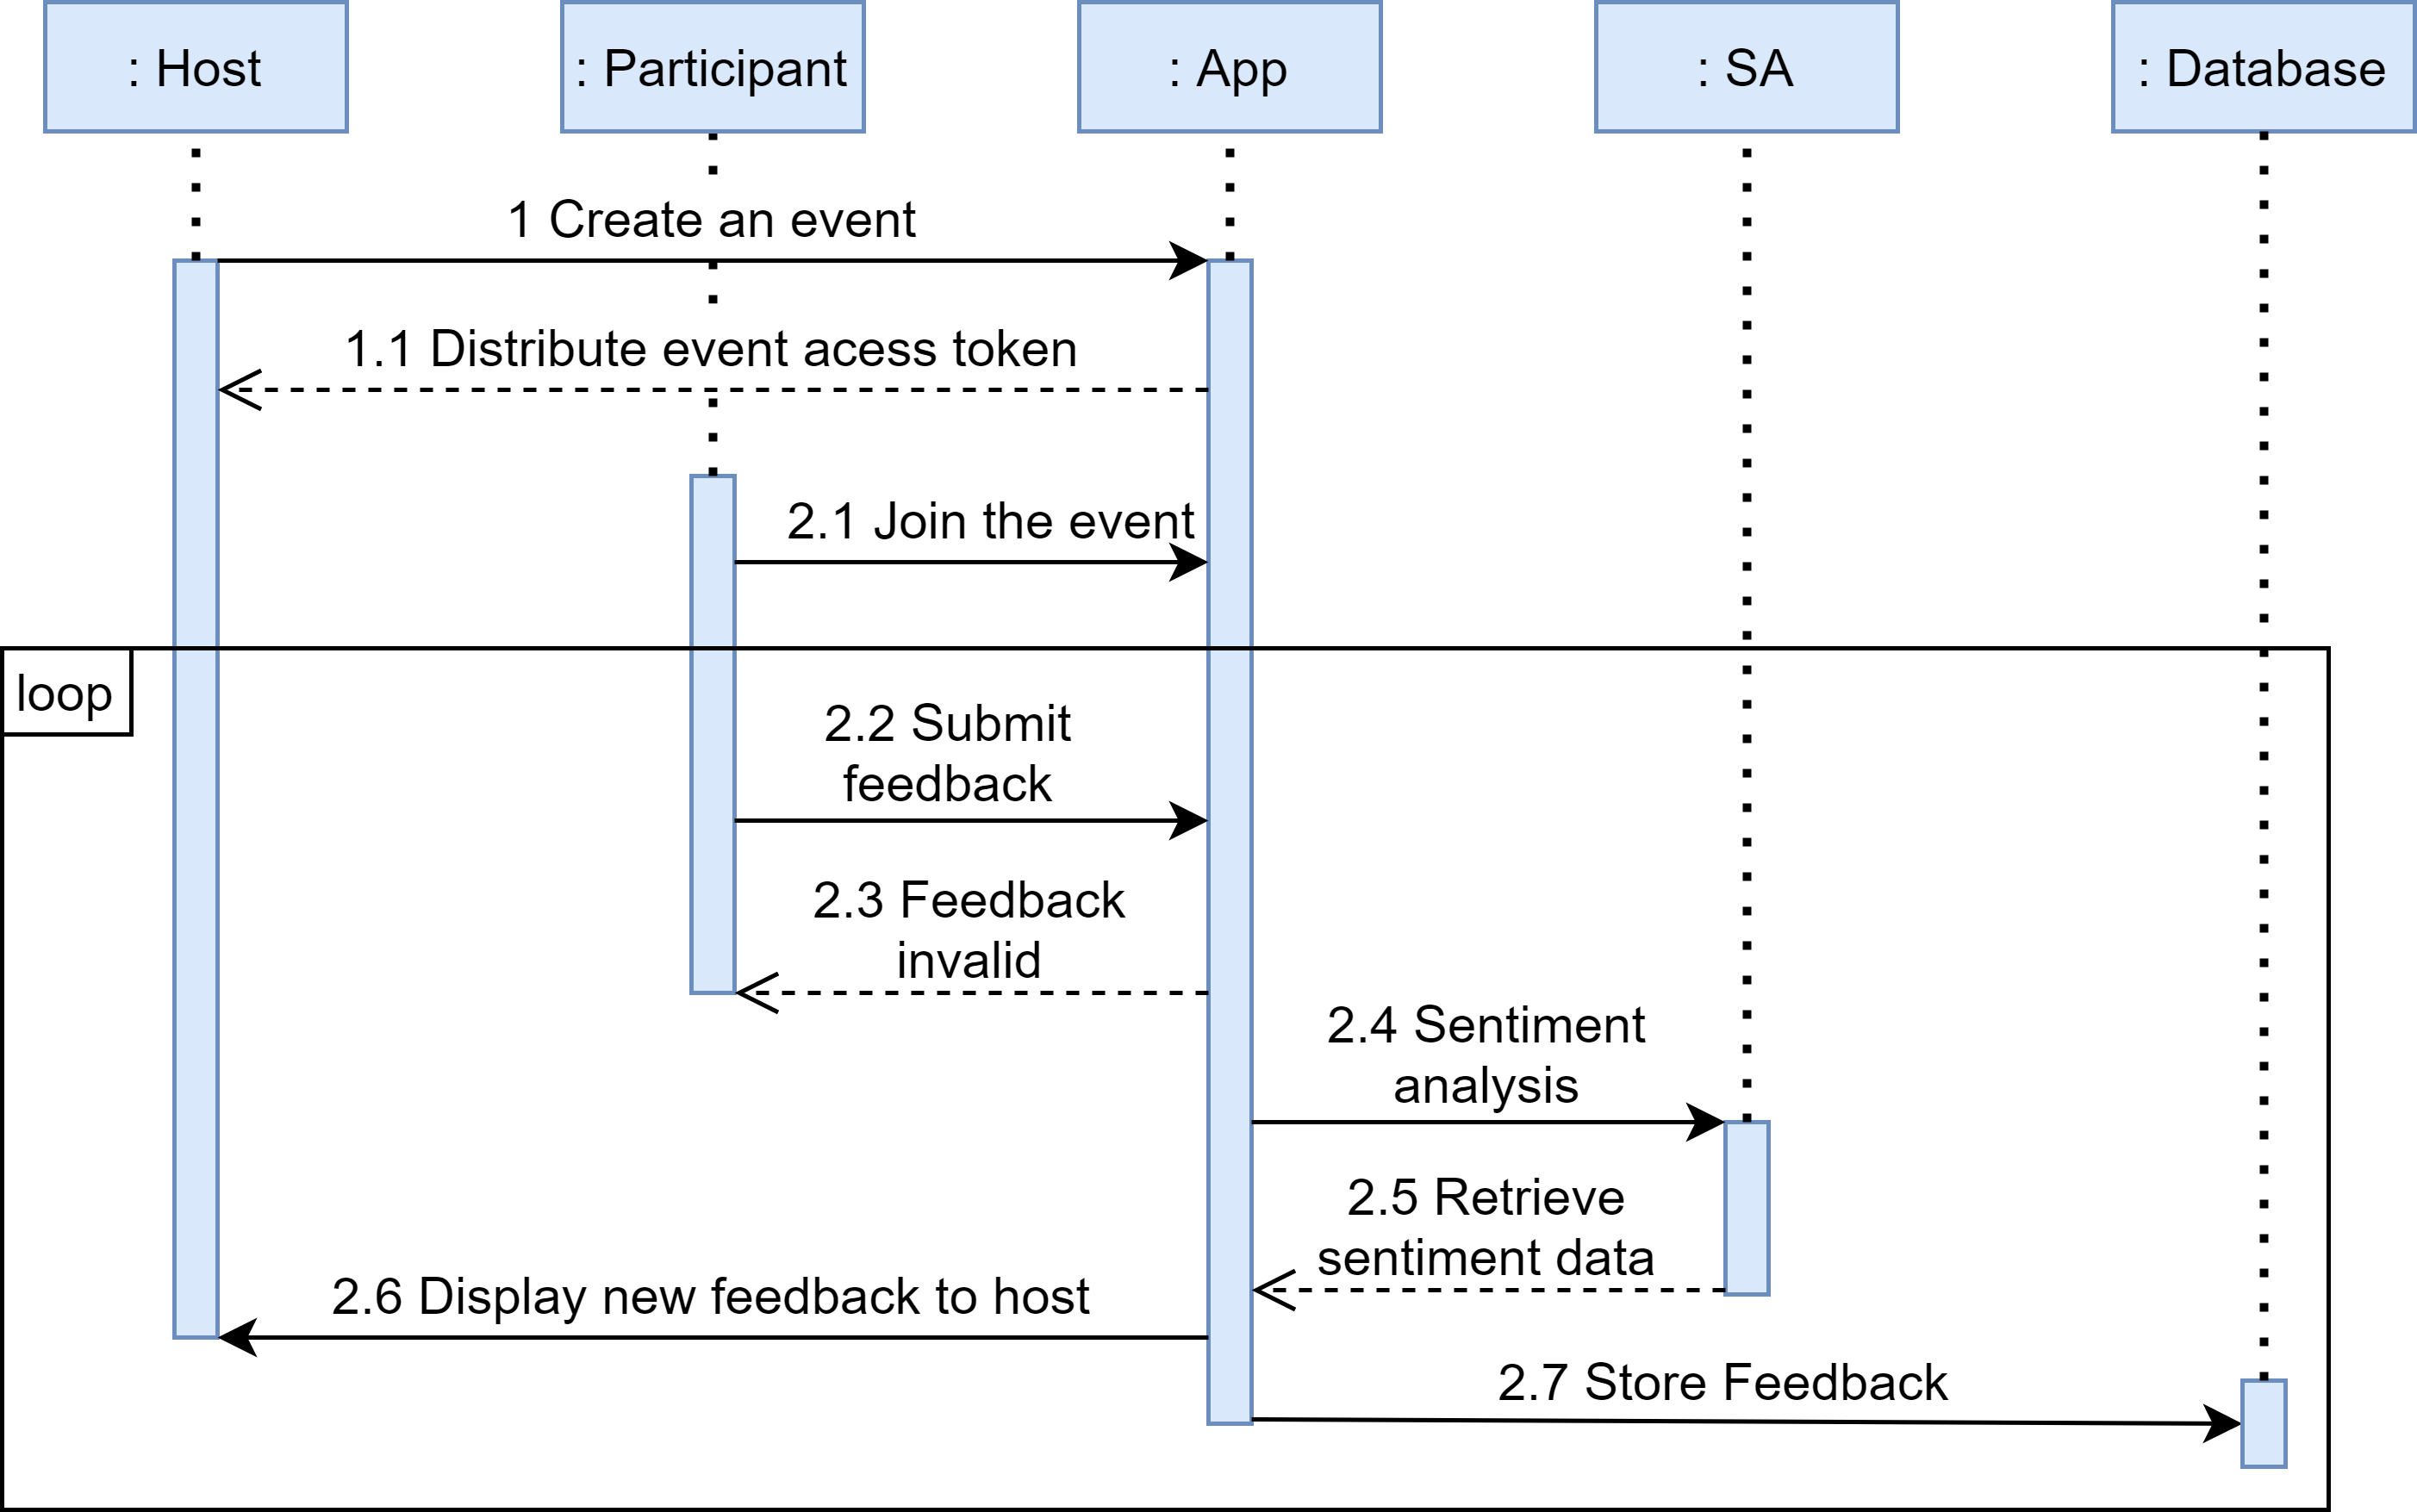
\includegraphics[width=0.6\textwidth]{assets/event-sequence.png}
\caption{An event sequence diagram (system-wide).}
\label{fig:sequence_diagram}
\end{wrapfigure}

\autoref{fig:sequence_diagram} shows the dynamic cooperation between multiple resources by describing the time sequence of messages sent between resources. Each box with a dotted line below represents a resource of that specific class. A solid line with an arrow represents a message to another resource, while a dotted line with a backwards arrow represents a reply from the other resource. The loop illustrates the process by which a participant interacts with an ongoing event. For example, at interaction 1 the host communicates with the web-app to create an event. The web-app then responds (interaction 1.1) by communicating the event access token. \autoref{fig:sequence_diagram} was created with Diagrams.net \autocite{web:drawio}.
\vspace{11mm}

\section{System Modelling}

\subsection{System Architecture}

\begin{figure}[!h]
  \centering
  \begin{minipage}[b]{0.49\textwidth}
    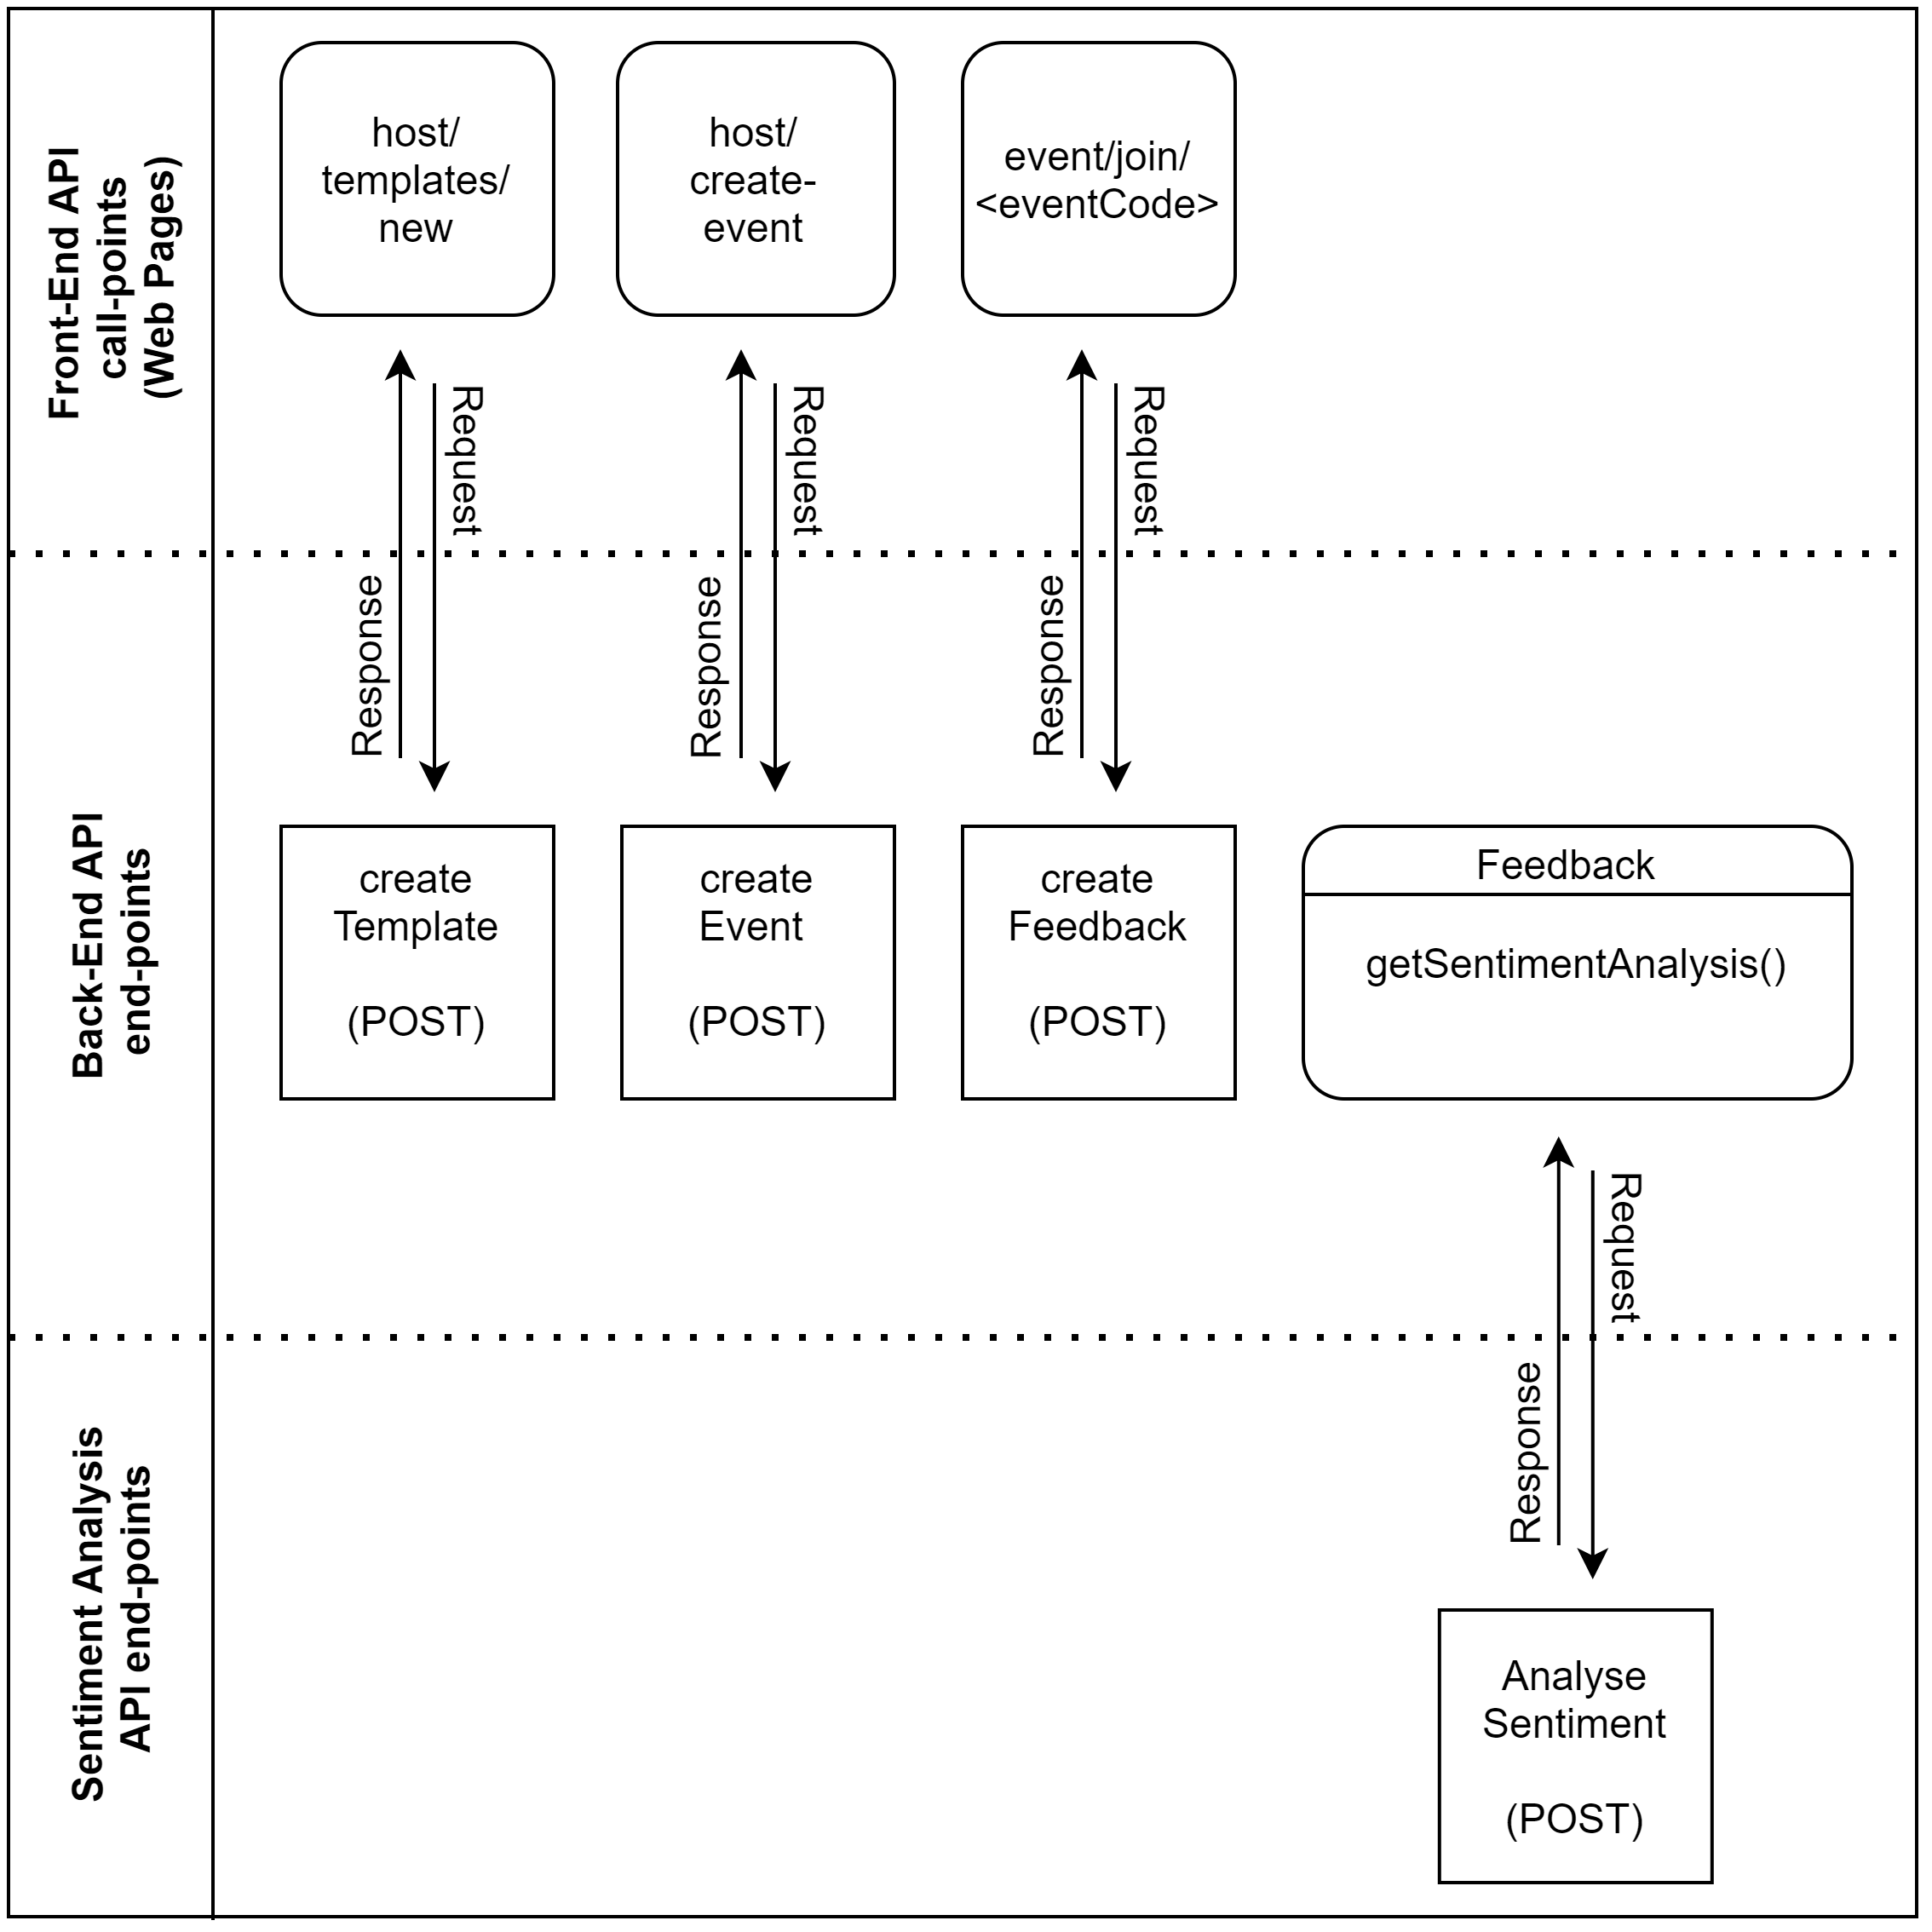
\includegraphics[width=\textwidth]{assets/REST_API.png}
    \caption{REST-API call-points and end-points, created with Diagrams.net \autocite{web:drawio}.}
\label{fig:apis}
  \end{minipage}
  \hfill
  \begin{minipage}[b]{0.49\textwidth}
    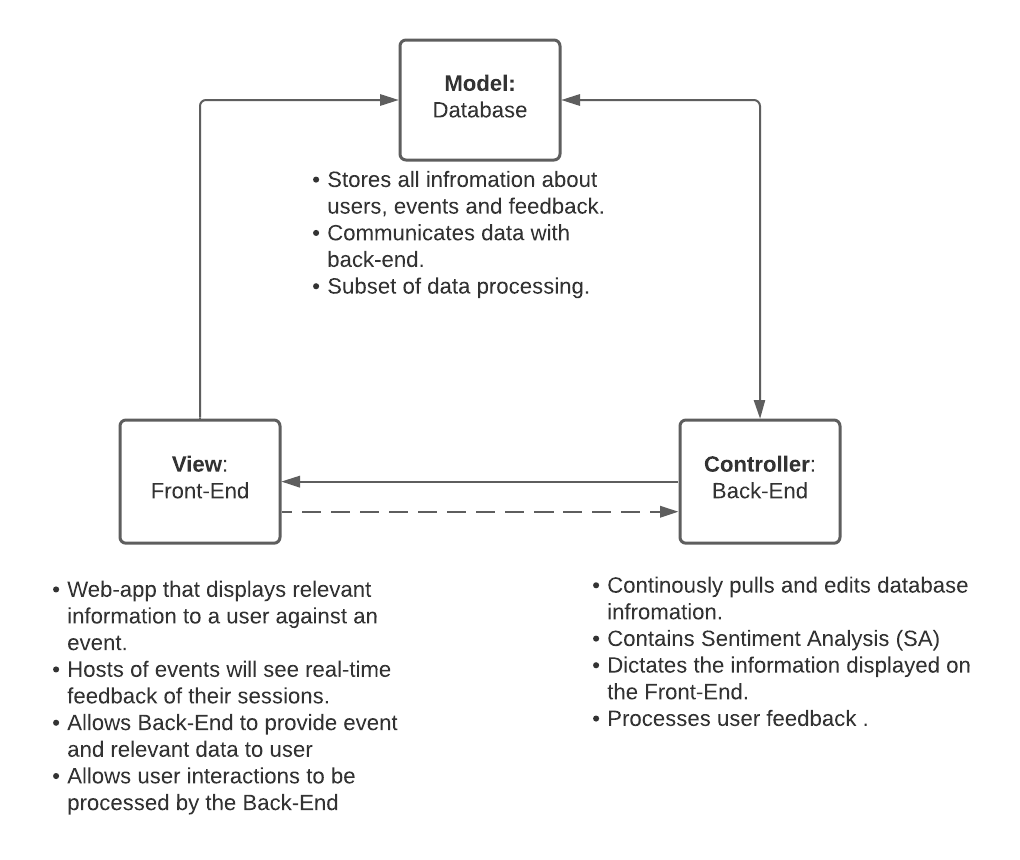
\includegraphics[width=\textwidth]{assets/mvc.png}
    \caption{A Model-View-Controller Architecture Diagram, created with Diagrams.net \autocite{web:drawio}.}
  \label{fig:mvc-diagram}
  \end{minipage}
\end{figure}

\textbf{Component Interaction: API Modelling}

\autoref{fig:apis} depicts a subset of the REST APIs within the proposed system. Rounded rectangles represent the API request (call) points, these are the site pages. Sharp rectangles represent the API response (end) points, responding to the requests launched by the call-points. Additional back-end API end-points include host creation and authentication. Each REST-API uses the POST method to communicate data (to keep uniform resource locators concise). \\

The Representational State Transfer API protocol (REST) was elected over alternative methods such as the SOAP protocol due to its decreased overhead and its reduced need for processing. 
This decreases system response latency, but does pose one disadvantage: the flexibility of data transmitted by REST API end-points can lead to invalid data. 
To ensure input validity, the system will validate API response and request objects. REST APIs are stateless meaning that API requests can be made independently - as a direct result, these APIs are also scalable, fulfilling [R:5.1-2].\\

\textbf{Web Sockets}\\
The back-end will establish a web socket connection between itself and the host within the host-facing event page. 
This connection will be used to communicate directly with the host, without the need for host-polling at some interval.
The use of web-sockets provides multiple benefits, the first of which being instant sending of feedback and event-related metrics to the host following feedback processing.
This means the system will provide the host with live feedback and updated event metrics in real time, meeting [R:13.1].\\

%%\newpage
\textbf{Model, View, Controller Design Pattern}

\autoref{fig:mvc-diagram} depicts the relationships between the back-end (Controller), the front-end (View) and Database (Model). The database can process its own data, and this data can also be accessed and manipulated by the back-end. The front-end corresponds to the web page the user interacts with. These interactions are processed by the back-end if necessary, with the database being updated upon a significant user interaction being processed.

%\newpage
\subsection{Component Modelling}

\textbf{Back-end Modelling} \label{back-comp-model}

\begin{figure}[h]
 \centering
 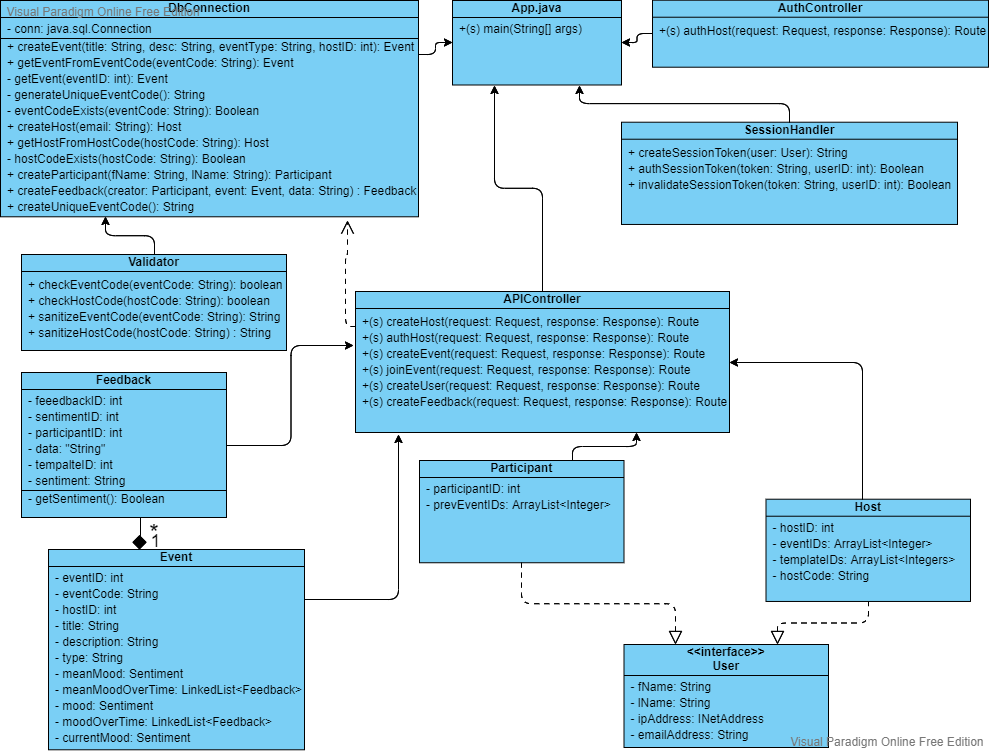
\includegraphics[width=\textwidth]{assets/be-classes.png}
 \caption{Back-End Class Structure, created with visual-paradigm.com \autocite{vp}}
 \label{fig:class-diagram}
 % MVC: {https://lucid.app/lucidchart/invitations/accept/cbc3f2a5-5c51-446b-a77b-88ed84abf628}
\end{figure}
 
\autoref{fig:class-diagram} illustrates the back-end structure with an overview of the classes that comprise it, with each class broken down into its components (attributes and methods). \texttt{DbConnection} holds all operations that handle and manipulate data from the database, and \texttt{APIController} holds the non-authenticating endpoints for the REST-APIs using the POST request method. The \texttt{Participant} and \texttt{Host} classes extend the interface \texttt{User}.\\

\textbf{Sentiment Analysis Modelling}\\
Sentiment Analysis is a process that utilises NLP on plain-text feedback, and queries with pre-defined inputs to produce a sentiment object. The sentiment object is composed of a real number variable (the approval rating), and sometimes some amount of string and/or real number variables (key results). Sentiment Analysis is derived from [R:12.1.D]. \newline

NLP is performed using the VADER framework. The VADER framework allows the solution to extract every discrete evaluative statement from a plain text string. Each statement is then broken down into words that match VADER's lexicon. Each word is then assigned a valence score, words are summed to create a valence score for the statement, and the score is then normalised between +1 (most positive) and -1 (most negative). This creates the compound score (a real number), a uni-dimensional measure of the statements evaluative disposition. A 3 value ratio is also generated, showing what fraction of the total statements are considered positive, negative, or neutral. A statement is categorised based on its normalised valence score (positive: compound score $\geq$ 0.05, negative: compound score $\leq$ -0.05, else neutral). This provides a multidimensional measure of the plain-text's evaluative disposition.\newline

The sentiment object contains an `approval metric' which is an overall estimation of the feedback's disposition. The approval metric is calculated from the weighted mean of various scores, normalised to a real number between 1 and -1 (as described above). The weighting and amount of scores will depend on the template used to submit feedback. Each score is derived from a distinct query within the template. Scores for each query will be derived either using NLP or by interpreting the one or more predefined inputs submitted by users. Not all queries within the template have to be considered when calculating the approval metric.\newline

Specific queries can also be designated as `key results' (this is not mutually exclusive with being weighted for the approval rating). These queries represent topics of feedback where the host desires easily accessible real time feedback. To be designated a key result a query must be limited to predefined inputs. This is to reduce ambiguity in data interpretation, and to more effectively provide summaries of complex topics for the host. Key results are held as string or real variables, depending on the query they relate to.\\

\textbf{Mood Modelling}

Mood is a temporal measure of the mean of every user's mean sentiment over a given period of time. To elaborate, mood is the mean of the mean sentiments of every instance of feedback with a common author submitted over a set period of time. For the total mood the period of time is the duration of the event. Calculating mood requires all the feedback to be submitted via the same template - this is always the case for any given event. Mood modelling is derived from [R:12.2.D]. \\

\textbf{Database Modelling}

\begin{figure}[h]
\centering
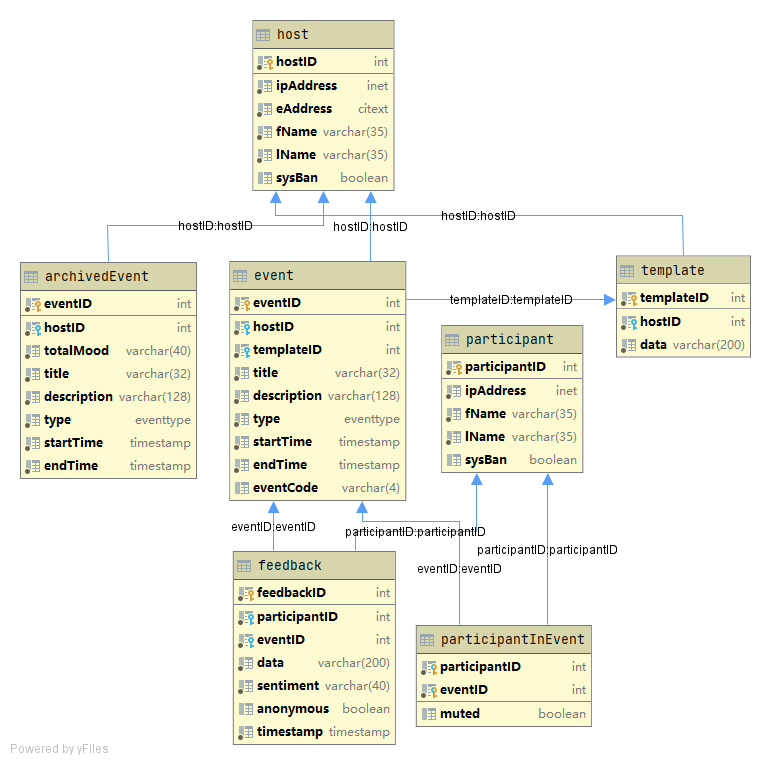
\includegraphics[width=0.75\textwidth]{assets/db.png}
\caption{Database Dependency Graph, created with DataGrip \autocite{dg}}
\label{fig:db-diagram}
\end{figure}

\autoref{fig:db-diagram} shows the relations and keys in the database. Hosts and participants are stored in separate relations so time is not wasted querying host objects from a table of all users. The template relation stores that template's creator's ID (\texttt{hostID}) which allows hosts to use previously created templates. The \texttt{ParticipantInEvent} relation links participants to their events and is used to reduce redundancy. These relations are in Third Normal Form - all the data elements in these relations are not only uniquely identified by the primary key but also independent of each other without any other functional relationship.\\

\textbf{Authentication} \label{auth}

The proposed solution makes use of host codes to authenticate hosts, and event codes to access events. This fulfills [R:4.2], [R:2.1], and [R:3.2], see below for implementation.\\

An event code is defined as a four digit, case-insensitive, alpha-numeric token, generated at event creation and unique to its event 
(e.g. Both \texttt{R2D2} and \texttt{c3po} are valid codes).
This provides the system with $(10+26)^4$ combinations, representing $1.68$ million unique event codes.
Event codes are to be distributed by the host (or their organisation) to all event participants. 
Participants can attend events either via a dynamic page URL (event/\texttt{<}eventCode\texttt{>}) or by entering the code on the landing page. Event URLs are dynamically deployed upon event creation.
Upon event archiving (a space-saving process on event completion), event codes are recycled by the system to minimise event-code saturation.\\

A host code is defined as a host-specific, private word set composed of four words, randomly chosen from a word list (e.g. \texttt{[Beans, Fish, Table, Moon]}). 
This provides the system with over 100 billion unique host codes. 
The system makes use of host codes to authenticate hosts, it assumes hosts are able to maintain the privacy of their codes.
While this method of authentication is well suited to the system as a proof of concept, any released product should change user authentication to a well implemented industry-standard compliant system, such as OAuth-2 \autocite{web:oauth}.\\

The \texttt{Validator} class exposes a set of methods to both sanitise, and assess the format validity of codes. \\
The \texttt{DbConnection} class exposes a set of methods to both create codes, and check their existence in the database.

%\newpage
\section{User Interface Design}

Figures \ref{fig:event_ui} and \ref{fig:template_ui} depict UI prototypes for event generation and template generation respectively. \newline
Both designs were produced using MockFlow \autocite{web:mockflow}. \newline

\textbf{Participant Event Page}
\begin{figure}[h]
\centering
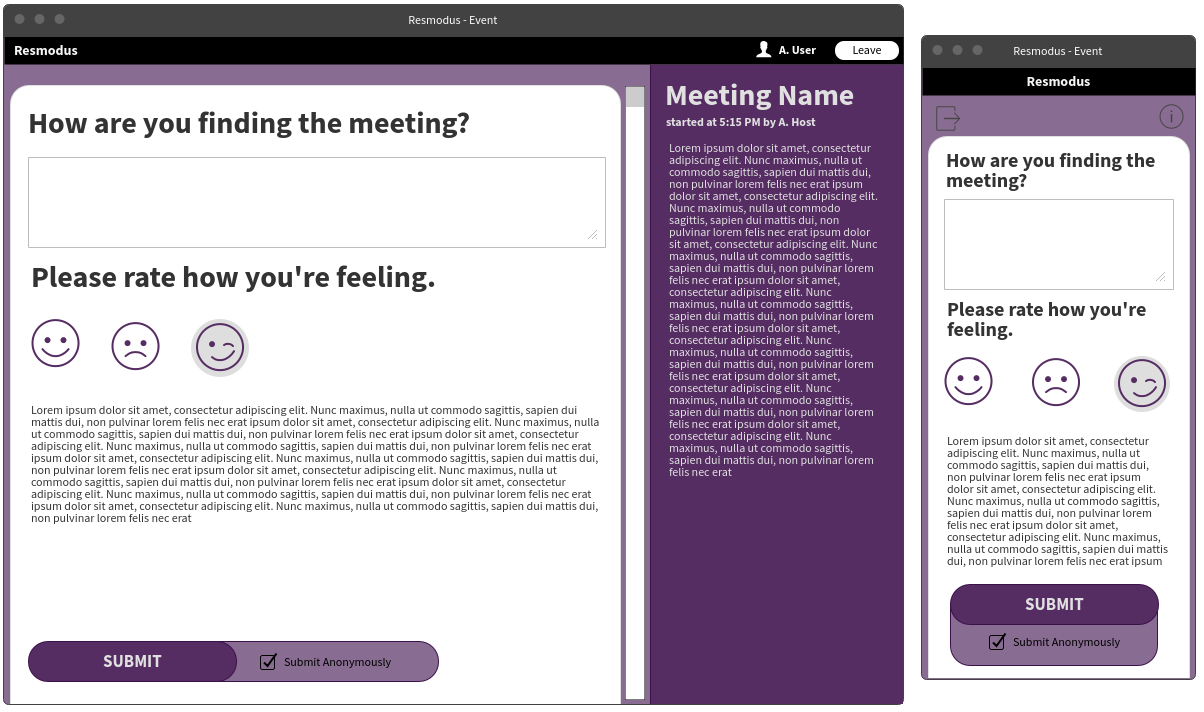
\includegraphics[width=0.75\textwidth]{assets/Event.png}
\caption{Mock-up of the Participant Event page for desktop (left) and mobile (right)}

\label{fig:event_ui}
\end{figure}

\autoref{fig:event_ui} shows the page viewed by participants upon joining an event. Participants can view meeting-related information in the right-hand sidebar on desktop, or by pressing the top-right icon on mobile. This page also contains a feedback submission form, in the form of the event-specific host-specified template. As can be seen in \autoref{fig:event_ui}, feedback instances can be marked as anonymous for anonymous submission. \newline

\textbf{Template Creation Page}
\begin{figure}[h]
\centering
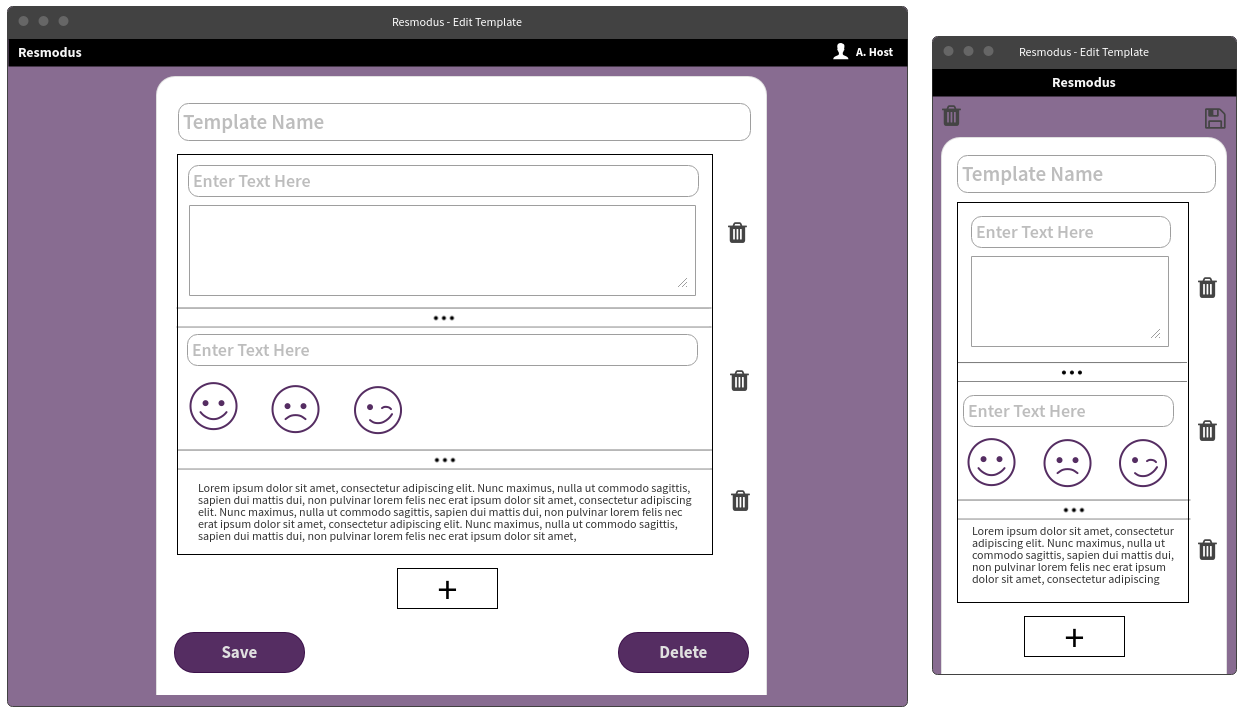
\includegraphics[width=0.75\textwidth]{assets/Template_Edit.png}
\caption{Mock-up of the Template Creation page for desktop (left) and mobile (right)}
\label{fig:template_ui}
\end{figure}

\autoref{fig:template_ui} shows the page viewed by hosts at template creation. Hosts can specify the template name, and add various components to the template - in this example a text input, a mood selector, and a paragraph of text have already been added. These components can be dragged around into the desired order, or removed by pressing the corresponding bin icon. The plus icon below the components will open a dialog allowing the host to select more components to add to the template. Hosts can either save or discard their template within template creation.

%%\newpage
\textbf{Application of GUI Design Principles}
% Application of GUI design principles (clarity, compatibility, comprehensibility, consistency, efficiency, familiarity, recovery, responsiveness, simplicity)

Loosely following rapid prototyping, research was conducted on existing products to inform the initial prototype. A pool of 11 potential users was then consulted, to qualitatively evaluate the first prototype (and following ones) and to suggest improvements. Potential users were first consulted individually, and then as a focus group. This was done to reap the benefits of collaborative discussions while mitigating the typical issues of bias and honesty among focus groups. At all stages of prototyping, industry-standard GUI design principles were followed strictly, specifically those described in `Principles of Effective Visual Communication for Graphical User Interface Design' \autocite{book:GUI1} and `Graphics in Human-Computer Communication: Principles of Graphical User-Interface Design' \autocite{book:GUI2}. The research methods described are derived from [R:9.1.D].\newline

The potential users found the most recent prototype (figures \ref{fig:event_ui} and \ref{fig:template_ui}) of the UI to be clear, comprehensible, and predictable. The prototypes were consistently styled and utilised principles of familiarity. An example being the use of `IBM defined globally recognisable button icons' \autocite{ibm}. The use of familiarity fulfills [R:6.1.C].\\

This prototype does not represent the finished solution's UI, but will instead serve as a basis for future development. As the design evolves the principles of interface design will be deeply considered to ensure user satisfaction and interface efficacy. This includes a focus on providing immediate acknowledgement for all user actions to promote responsiveness. Transitions between controls and the minimisation of user hand and eye movements must also be considered to ensure interface efficiency. Ensuring efficiency contributes to [R:5.1.C].

%%\newpage
\section{Design Considerations}

\textbf{Extensibility}\\
The principle of extensiblity is concerned with future growth, and the effort required to implement said growth. A primary concern is enhancing the solution without impairing existing functions. This has already been considered in the Requirements Analysis, where implementation prioritisation was used to propose low priority functional requirements. These requirements (while not likely to be implemented) represent documented and validated areas for growth, should the project find the opportunity to invest in them. \\

Our proposed solution minimises technical debt, reducing the difficulties in extending the project. Future back-end services, such as new APIs, can be added to the back-end. For the system front-end, React's components allow for ease of edibility without loss of structure. The addition of new pages to the system would also be supported.\\

% TA Approved
\textbf{Robustness}\\
Robustness is a measure of the system's ability to tolerate unpredictable or invalid inputs. 
The system collects user input in the following sub-systems: feedback submission, entering event codes, entering host codes, creating templates, and submitting event related data such as title and description. 
Users use URLs to access system pages. Non-defined system pages will render 404 errors upon user access, and previously defined pages such as completed events will inform the user that said event is finished, followed by a redirect to the landing page. Both the front-end and back-end will implement user input control: the front-end through constraining form data types, and the back-end by implementing sanitisation checks against user-defined codes (host, template, and event codes). See the \texttt{Validator} class in \hyperref[back-comp-model]{[back-end modelling]}. The API endpoints will ensure correct types for request fields, for each request. \\


\textbf{Reliability}\\
Reliability is a measure of how well the system performs under everyday conditions. The reliability of the system will be measured through the consistency of the feedback processing speed. The speed of feedback processing should remain unaffected by the rise of user population. This will be achieved as sentiment analysis is abstracted to an API, allowing for scalability with respect to server infrastructure. \\


\textbf{Correctness}\\
Correctness is how accurately the solution meets the requirements of the customer. Correctness can be considered both at the point of design, and continually through the development process. Within this design document, system components have been linked with the set of requirements they fulfill. These requirements are traceable to specific customer requests and/or their implications. Following this process ensures the design is necessary and correct.\\

Upon sprint cycle initialisation: traceable, necessary, and correct requirements shall be generated. At sprint cycle review \hyperref[methodology]{[see methodology]} the developed components shall be traced to the requirements from which they are derived, checking their correctness. Through this approach the scrum methodology ensures correctness is maintained throughout the project.\\ 

\textbf{Compatibility and Portability}\\
Compatibility and portability are concerned with the installation and execution of the solution. 
Our web-client is cross-platform accessible: the user requires no dedicated native app, only a compatible browser, and a stable internet connection (see Requirements Analysis, Assumptions). The solution is also accessible via a mobile app on Android and iOS. The choice of React, with the use of React Native on mobile,  makes mobile development labour economical. The back-end software is also versatile due to the use of Java, which can be ported to any system supporting the Java Run-time Environment (JRE). High portability contributes to [5.2.C]. \\

\textbf{Modularity and Reuse}\\
% how well your system is divided into independent components and whether you have reused existing code;
Both the front-end and back-end are designed in a modular way - they can be changed given that the changes mirror the back-end services provided (API and sockets), and given that the changes to the front-end interact with the same API endpoints. Given that the web-app is written in React and the mobile version is written in React Native, large amounts of the React code can be shared and reused between platforms. \\

\textbf{Security}\\
A truly robust security policy is beyond the scope of this project. The projects approach towards low level attacks and hostile misuse is documented under [R:14.1-5] and [R:4.2] respectively. These requirements list several risk mitigating features. In addition to these the host code \hyperref[auth]{[authentication]} system provides an excess of 100 billion host codes, this significantly reduces the feasibility of a malicious user guessing an active host code.\\

\textbf{Fault-tolerance}\\
% whether your system can withstand hostile acts and influences;
The system abstracts back-end interaction into APIs, meaning API failures are independent of each other - only the API that fails is effected. For redundancy, multiple API response servers can be launched upon deployment, serving a duplicated set of services. Fault-tolerance is derived from [R:4.1.D] and [R:6.2].

\section{Testing and Validation}
% You need to show how you will validate your system.
% There should be a robust test plan, and it should be linked to your requirements.
% You need to show that the system will meet the customer’s needs.
% Just saying ‘’re doing unit testing’ is bad.

\subsection{Unit Testing}

Throughout the project unit testing will be used to validate the correctness of solution components, and to ensure requirement fulfillment. These unit tests will be developed before the code they are assessing, and unit tests are defined for each back-end task against the sprint cycle backlog; in some cases, these represent requirements. Unit tests can be performed against back-end systems, such as: API end-points, the database, and sentiment analysis, as well as the standard back-end methods. With database testing, the solution will implement standardised security testing frameworks to assess the system's risk to SQL injection attacks.

\subsection{System Testing}

Following core development cessation, the solution is subject to system testing to assess correctness, robustness, and to ensure project requirements are fulfilled. System testing will be performed in sprint cycle five, throughout project week eight.\\

\textbf{User Acceptance Testing}\\
One such system testing technique is that of user acceptance testing. The user experience will be tested using eight simulated users with no prior knowledge of the system. Each simulated user is assigned a set of tasks to complete, user responses, behaviour and system-metrics are all recorded. Following the tests the users answers a survey on their experience. This is combined with the metrics recorded during their test to produce the `User Acceptance Summary'. The summary records the key data reported by every user. This includes: time to learn, reported difficulties, ratings on intuitiveness and ease of use, common mistakes, ratings on the solutions mistake avoidance, latency, failures and ambiguities in the solution, design ratings and comments, and potential improvements to the solution. The user acceptance summary is then evaluated to determine the results of the tests. This is derived from and fulfills [R:4.3.D]\\

\textbf{Front-end and UI testing}\\
Device-compatibility testing will be performed to evaluate the design and responsiveness of the web-page, assessing its behaviour and structure at different screen sizes and on different devices. The whole page structure will be explored to check for styling errors (for example miss-aligned text). The solution can also be tested for web-standard compliance, using the W3C Markup Validator \autocite{web:w3c}. \\

\textbf{Complexity Analysis and Reliability Testing}\\
The solution will have its estimated worst case time and space complexity determined. This serves to satisfy [R:5.1.D], and to assess if the solution is efficient and performant (see [R:5.1]). Additionally, space complexity will assist in assessing the solution's scalability as outlined in [R:6.2]. The solution will be tested to determine if it can run continuously for 5 days (longest continuous period of working days in a year). This is derived from [R:6.2.D].

%\newpage
\section{Planning}

\textbf{Methodology} \label{methodology} \newline
The project team will use Scrum \autocite{web:scrum}, an Agile framework \autocite{web:agile} with fixed deadlines for project closure; this better aligns the project with the client's needs. 
Strong customer involvement is key to agile methodologies, and Scrum allocates a Scrum Master to interface with the customer: the elected scrum master is {Alexander}. 
Work is performed in weekly sprint cycles, completing items from a backlog of work against the component in development. \autoref{fig:gantt} outlines the project sprint cycles. Each sprint cycle backlog will be placed on an online, collaborative Kanban board - see Trello \autocite{web:trello}.
Scum meetings will be held three times each week, at 10 am to noon, on Mondays, Wednesdays, and Fridays. Before development, meetings were held bi-weekly on Tuesdays and Thursdays, both at 10 am to noon. Sprint Reviews allow the team to both present work and assess it by quality and within the context of project progress. \newline

\textbf{Decision Making}\newline
Wider-scope project decisions are considered in group meetings by all members. When there is no consensus, the project manager holds the decisive vote.
Component-specific decisions are also considered by all members, within sprint cycle meetings. Without consensus, the development lead makes the final call.
For example, in the case of a front-end related dispute, the front-end technical lead ({George}) would have the decisive vote. \newline

% ---- JUSTIFICATION ----
\textbf{Justification}\newline
Agile was chosen for its adaptability to specification changes, and by extension, requirement changes. 
Scrum’s sprint cycles provide a logical approach to breaking down development, and sprint reviews allow the team, and the client, to see tangible project-progress. These reviews also provide a point of reflection against the project, allowing for changes to be made to the pace of development to ensure project closure by the client-imposed strict deadline. 
Having a scrum master allows for abstracted client involvement, allowing the solution to better align with the client's vision. 
The benefits of adaptability and customer-focus are not key components of plan-based approaches, hence the decision to use an Agile framework.
Various adaptive methods were considered, such as rapid application development and agile test-driven development, but Scrum was favoured due to its superior management of client involvement, more logical and appropriate breakdown of development, and code review framework. One caveat of the Scrum methodology is the need for frequent, in-person team meetings to discuss current work. These in-person meetings will be simulated by online video meetings. As some members are overseas, there is a restricted window for scrum meetings. \newline

% ---- SPECIFICS ----
% Split into: Product Backlog, Sprint Backlog, Increment\\

\textbf{Logistics} \label{group:logistics}

\begin{figure}[h!]
    \centering
    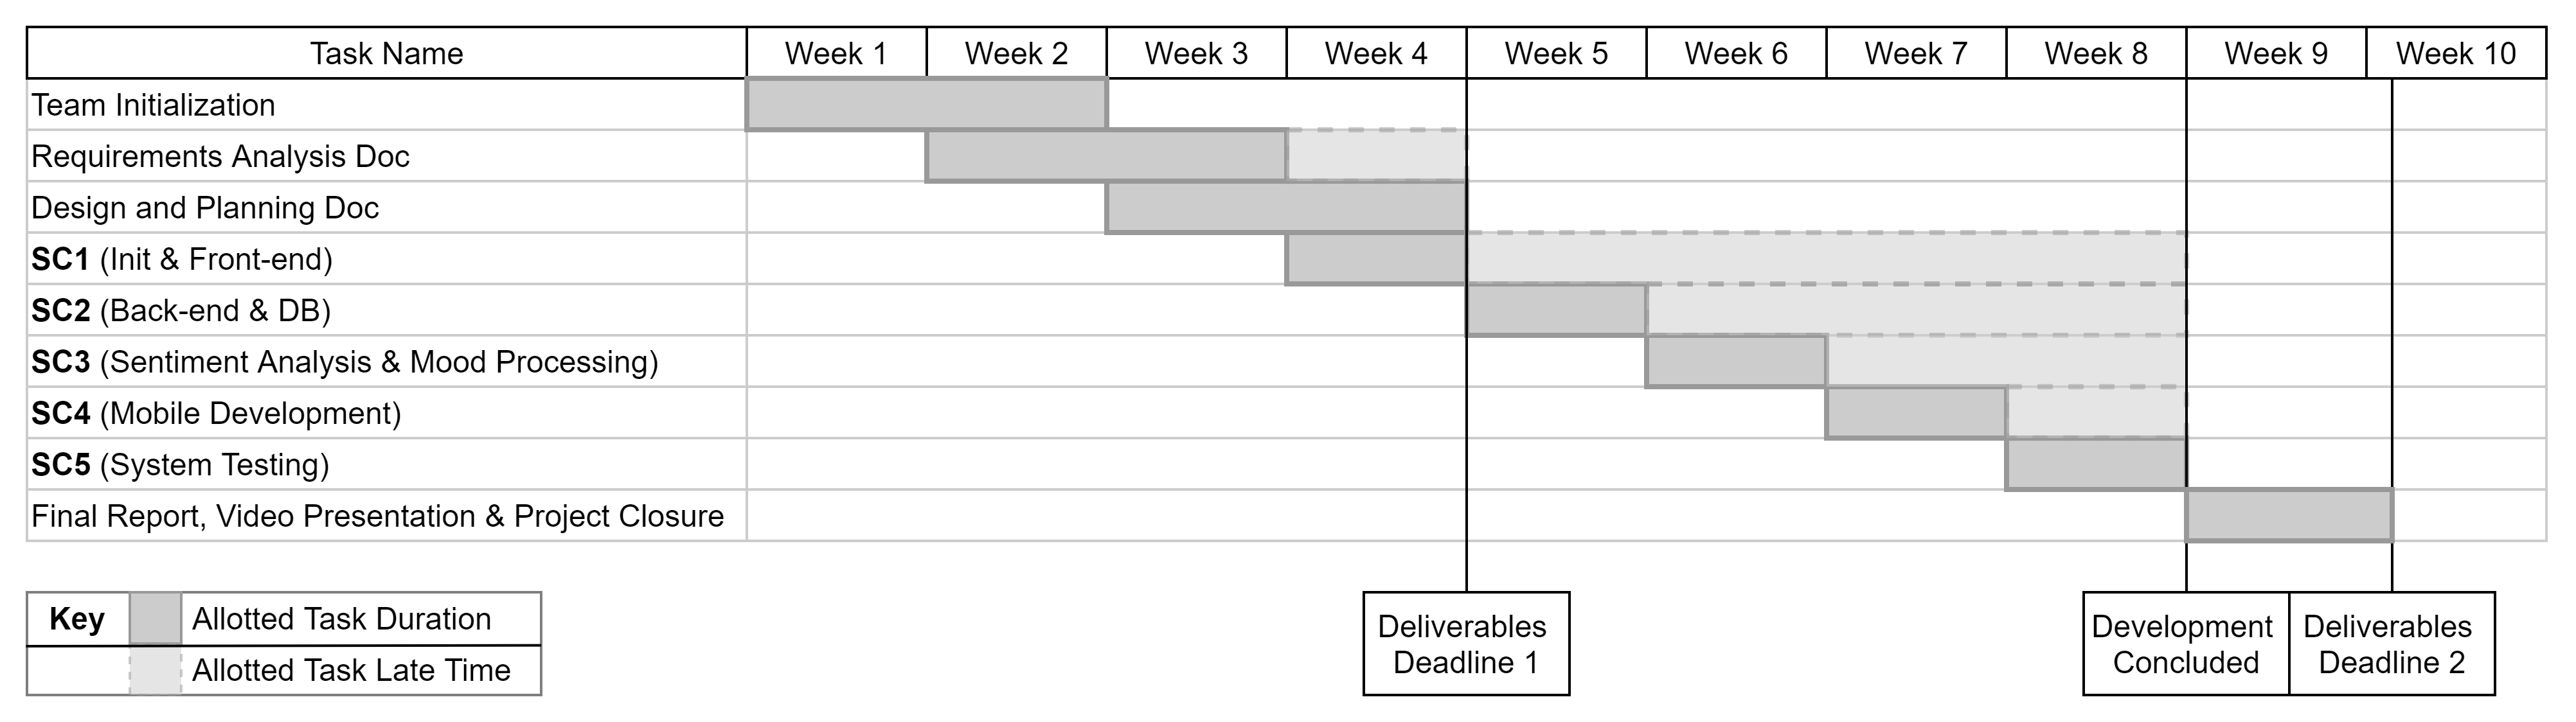
\includegraphics[width=\textwidth]{assets/gantt.png}
    \caption{Gantt Chart of Project Schedule, created with Diagrams.net \autocite{web:drawio}}
    \label{fig:gantt}
\end{figure}

A critical path analysis graph was considered, but due to the adaptability of the methodology, it was found to be of limited usefulness.\\


The project's Sprint Review Framework considers the following questions: 
\begin{itemize}[noitemsep, topsep=0pt, leftmargin=12mm]
 \item[Q1: ] Does code conform to maintenance practices outlined in \hyperref[sec:req:nf]{non-functional requirement five}? 
 \item[Q2: ] Have changes been made to the underlying specification since the previous review? 
 \item[Q3: ] Is the rate of development sufficient to meet deadlines? 
\end{itemize}

%\newpage
\section{Risk Analysis}
It is important to consider the risks involved in a project of this scale, and to ensure that they are prepared for. Below is a risk register identifying possible project risks, their likelihood of occurring, their potential impact on the project, mitigation plans, and the residual risk following rectification.

\begin{center}
    \begin{tabular}{|m{5cm}|m{1.8cm}|m{1.2cm}|m{4.5cm}|m{1.5cm}|}
    \hline
        \vspace{1mm}
        \textbf{Risk} & \textbf{Likelihood} & \textbf{Impact} & \textbf{Treatment} & \textbf{Residual Risk}  \\
        \hline
        Team member is partially or fully unable to contribute with a reasonable justification given &
        Medium &
        Medium &
        Notify other members and delegate affected work &
        Low \\
        \hline
        Member neglects responsibilities without a reasonable justification &
        Low &
        Medium &
        PM reminds member of responsibilities and possibly pursues further action (re-delegation of work) &
        Low \\
        \hline
        Project creep (client wishes to make changes midway through the project) &
        High &
        Medium &
        Use an adaptable framework &
        Low \\
        \hline
        Dependency on specific members for specific components &
        Medium &
        Medium &
        Have all members contribute to all components &
        Low \\
        \hline
        Data loss due to hardware fault &
        Low &
        High &
        Use of version control with regular commits to update work &
        Medium \\
        \hline
        Project termination by client &
        Low &
        High &
        N/A &
        High \\
         %project creep - stakeholder wants to make changes midway through project
         \hline
    \end{tabular}
\end{center}

\printbibliography[heading=bibintoc]

\end{document}


% DB SCHEMA FIRST DRAFT (YANG)
% \textbf{Database Schema (draft) - diagram supersedes this}
% \vspace*{2mm}
% \hline
% \begin{center}\begin{tabular}{ll}
%     \textbf{Table Name} & \textbf{Table Attributes} \\
%     User & UserID, FName, LName, EmailAddress, (Password)\\
%     Event & EventID, Name, Description, HostID, EventCode\\
%     Feedback & FeedbackID, UserID, Content, Mood, Sentiment\\
%     Template & TemplateID, EventID, Content\\
%     UserInEvent & UserID, EventID\\
%     FeedbackInEvent & FeedbackID, EventID\\
% \end{tabular}\end{center}
% \vspace*{-2mm}\hline

% \vspace*{2mm}\hline\vspace*{-1.5mm}
% \begin{center}\begin{tabular}{lll}
%     \textbf{Sprint Cycle} & \textbf{Time Period} & \textbf{Main System Components}\\
%             % & Weeks 1-2 & Group Meeting and Organisation \\
%             % & Week 3 & Requirements Analysis and Design \\
%     Cycle 1 & Week 4 & Project Initialisation and Front-end \\
%     Cycle 2 & Week 5 & Back-end Functionality and Database \\
%     Cycle 3 & Week 6 & Sentiment Analysis \\
%     Cycle 4 & Week 7 & Mobile Development \\
%     Cycle 5 & Week 8 & System Testing 
%             % & Week 9 & VIDEO, REPORT \\
%             % & Week 10 & MONDAY IS DEADLINE
% \end{tabular}\end{center}
% \vspace*{-2mm}\hline\vspace*{2mm}